%!TEX ROOT=main.tex


\chapter{Personal development domain}\label{ch:personal-development-domain}


This section will introduce the reader to the domain of personal development.
Justification of the idea behind the application will also be presented here.

%Use empirical statements


\section{Definition of personal development}\label{sec:definition-of-personal-development}

In order to create helpful application, it is crucial to build it based on principles and ideas of personal development.
Familiarisation with these will start from the definition of personal development and with Maslow's hierarchy of needs in particular.

\begin{figure}[h]
    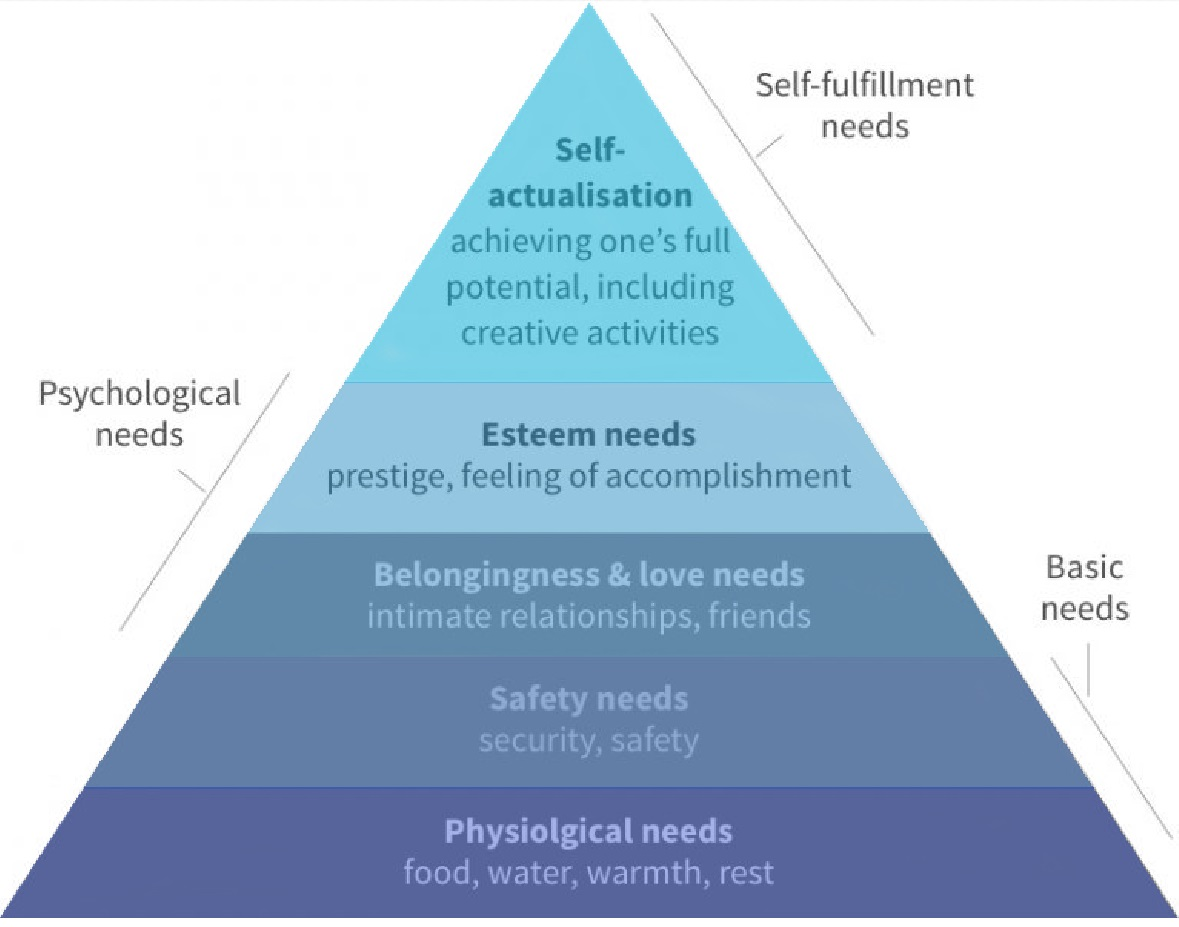
\includegraphics[width=0.75\textwidth]{images/maslows.jpg}
    \caption{Maslow's Hierarchy of Needs~\cite{maslows}}
    \label{fig:maslows}
\end{figure}

The pyramid shown in figure~\ref{fig:maslows} might be familiar to the reader.
Going from the bottom to the top, the first two levels are basic needs that every person needs the most.
The following two levels are psychological needs, that comes after physical ones.
It may be presumed, that a person has satisfied lower levels before beginning to satisfy the higher levels.
At the top of the pyramid is the need for "self-actualisation".
Self-actualisation refers to the desire of reaching one's full potential and could be considered as the goal and motivator for the process of personal development.
As pyramid contains highly relatable needs, it is safe to assume that the need for self-actualisation will be known to the reader.

Personal development is the set of activities aimed at enhancement of employability, improvement of quality of life and raising one's confidence ~\cite{what-is-personal-development}.
Motivation for personal development comes from the need for self-actualisation and thereby makes it a natural and relatable feeling.





Personal development then could be described as the process of reaching one's full potential.
This definition includes many ways of interpretation, since each could describe their "potential" differently.



Only with the first two levels fulfilled, comes need
After the fulfillment of these needs
It has basic physiological needs at the bottom, psychological needs in the middle and self-realisation needs at the top.
It


It is fair to say, that each person could give own definition of personal development.
It is nesse
It requires no special knowledge to define what personal development is.

Every person is aware of the concept of personal development.
The process of personal development is natural.
